% Send in the clones? - Journal club Cars (2026) doi:10.1002/pds.70354
% (c) 2026 Malcolm Gillies <malcolm.gillies@unsw.edu.au>
% https://github.com/mbg-unsw/send-in-the-clones
%
% This work is licensed under a
% Creative Commons Attribution-NonCommercial-ShareAlike 4.0
% International Licence
\documentclass[aspectratio=169,12pt]{beamer} % XXXX fix AR here
\usepackage{pgfpages}
\usepackage{fancyvrb}
\usepackage{pgfplots}
%\usepackage[latin1]{inputenc}
%\usepackage[T1]{fontenc}
%\usepackage{textcomp}
%\usefonttheme{serif} % need this with Charter font
\usetheme{auriga}  % using default now
\usecolortheme{auriga}  % using default now
%\usepackage[libertine]{libertine} % not using osf (old-style figures)
%\usepackage[scale=0.9]{tgheros} % scale to match libertine
%\usepackage[varqu,varl]{inconsolata}
%\usepackage[libertine]{newtxmath}
\usepackage{graphicx}
\usepackage{tikz}
\usetikzlibrary{shadows}
\usepackage{tikzpagenodes}
\usepackage[round]{natbib}
\usepackage{gitinfo2}
\usepackage{booktabs}

\pgfplotsset{compat=1.17}
\hypersetup{pdfencoding=auto}

\renewcommand{\gitMark}{\color{lightgray}\texttt{\tiny\gitBranch\,@\,\gitAbbrevHash\,\gitAuthorDate}}

%\renewcommand{\bibsection}{} % suppress "References" section

%\setbeamertemplate{navigation symbols}{} % remove navigation symbols
%\setbeamercolor*{item}{fg=darkred}

\title{Send in the clones? Challenges in emulating a trial of PCSK9 inhibitor treatment}
\author{Malcolm Gillies <malcolm.gillies@unsw.edu.au>}
\institute{VAC4EU Journal Club\\18 September 2026}
\usebackgroundtemplate{%

\includegraphics[width=\paperwidth]{ref/micre-blank.PNG}
\begin{tikzpicture}[remember picture,overlay]
    \node[anchor=south east,scale=1,rotate=90] at ([shift={(0cm,0cm)}]current page marginpar area.north east) {\gitMark};
\end{tikzpicture}%
}


\newif\ifsidebartheme
\sidebarthemefalse

\newdimen\contentheight
\newdimen\contentwidth
\newdimen\contentleft
\newdimen\contentbottom
\makeatletter
\newcommand*{\calculatespace}{%
    \contentheight=\paperheight%
    \ifx\beamer@frametitle\@empty%
        \setbox\@tempboxa=\box\voidb@x%
      \else%
        \setbox\@tempboxa=\vbox{%
          \vbox{}%
          {\parskip0pt\usebeamertemplate***{frametitle}}%
        }%
        \ifsidebartheme%
          \advance\contentheight by-1em%
        \fi%
      \fi%
    \advance\contentheight by-\ht\@tempboxa%
    \advance\contentheight by-\dp\@tempboxa%
    \advance\contentheight by-\beamer@frametopskip%
    \ifbeamer@plainframe%
    \contentbottom=0pt%
    \else%
    \advance\contentheight by-\headheight%
    \advance\contentheight by\headdp%
    \advance\contentheight by-\footheight%
    \advance\contentheight by4pt%
    \contentbottom=\footheight%
    \advance\contentbottom by-4pt%
    \fi%
    \contentwidth=\paperwidth%
    \ifbeamer@plainframe%
    \contentleft=0pt%
    \else%
    \advance\contentwidth by-\beamer@rightsidebar%
    \advance\contentwidth by-\beamer@leftsidebar\relax%
    \contentleft=\beamer@leftsidebar%
    \fi%
}
\makeatother

\begin{document}

%\setbeamercolor{page number in head/foot}{fg=white}
%
%{
%\usebackgroundtemplate{
\includegraphics[width=\paperwidth]{ref/micre.PNG}}
%\setbeamercolor{title page}{fg=white}
%  \begin{frame}[plain]
%    \titlepage
%  \end{frame}
%}

{
\usebackgroundtemplate{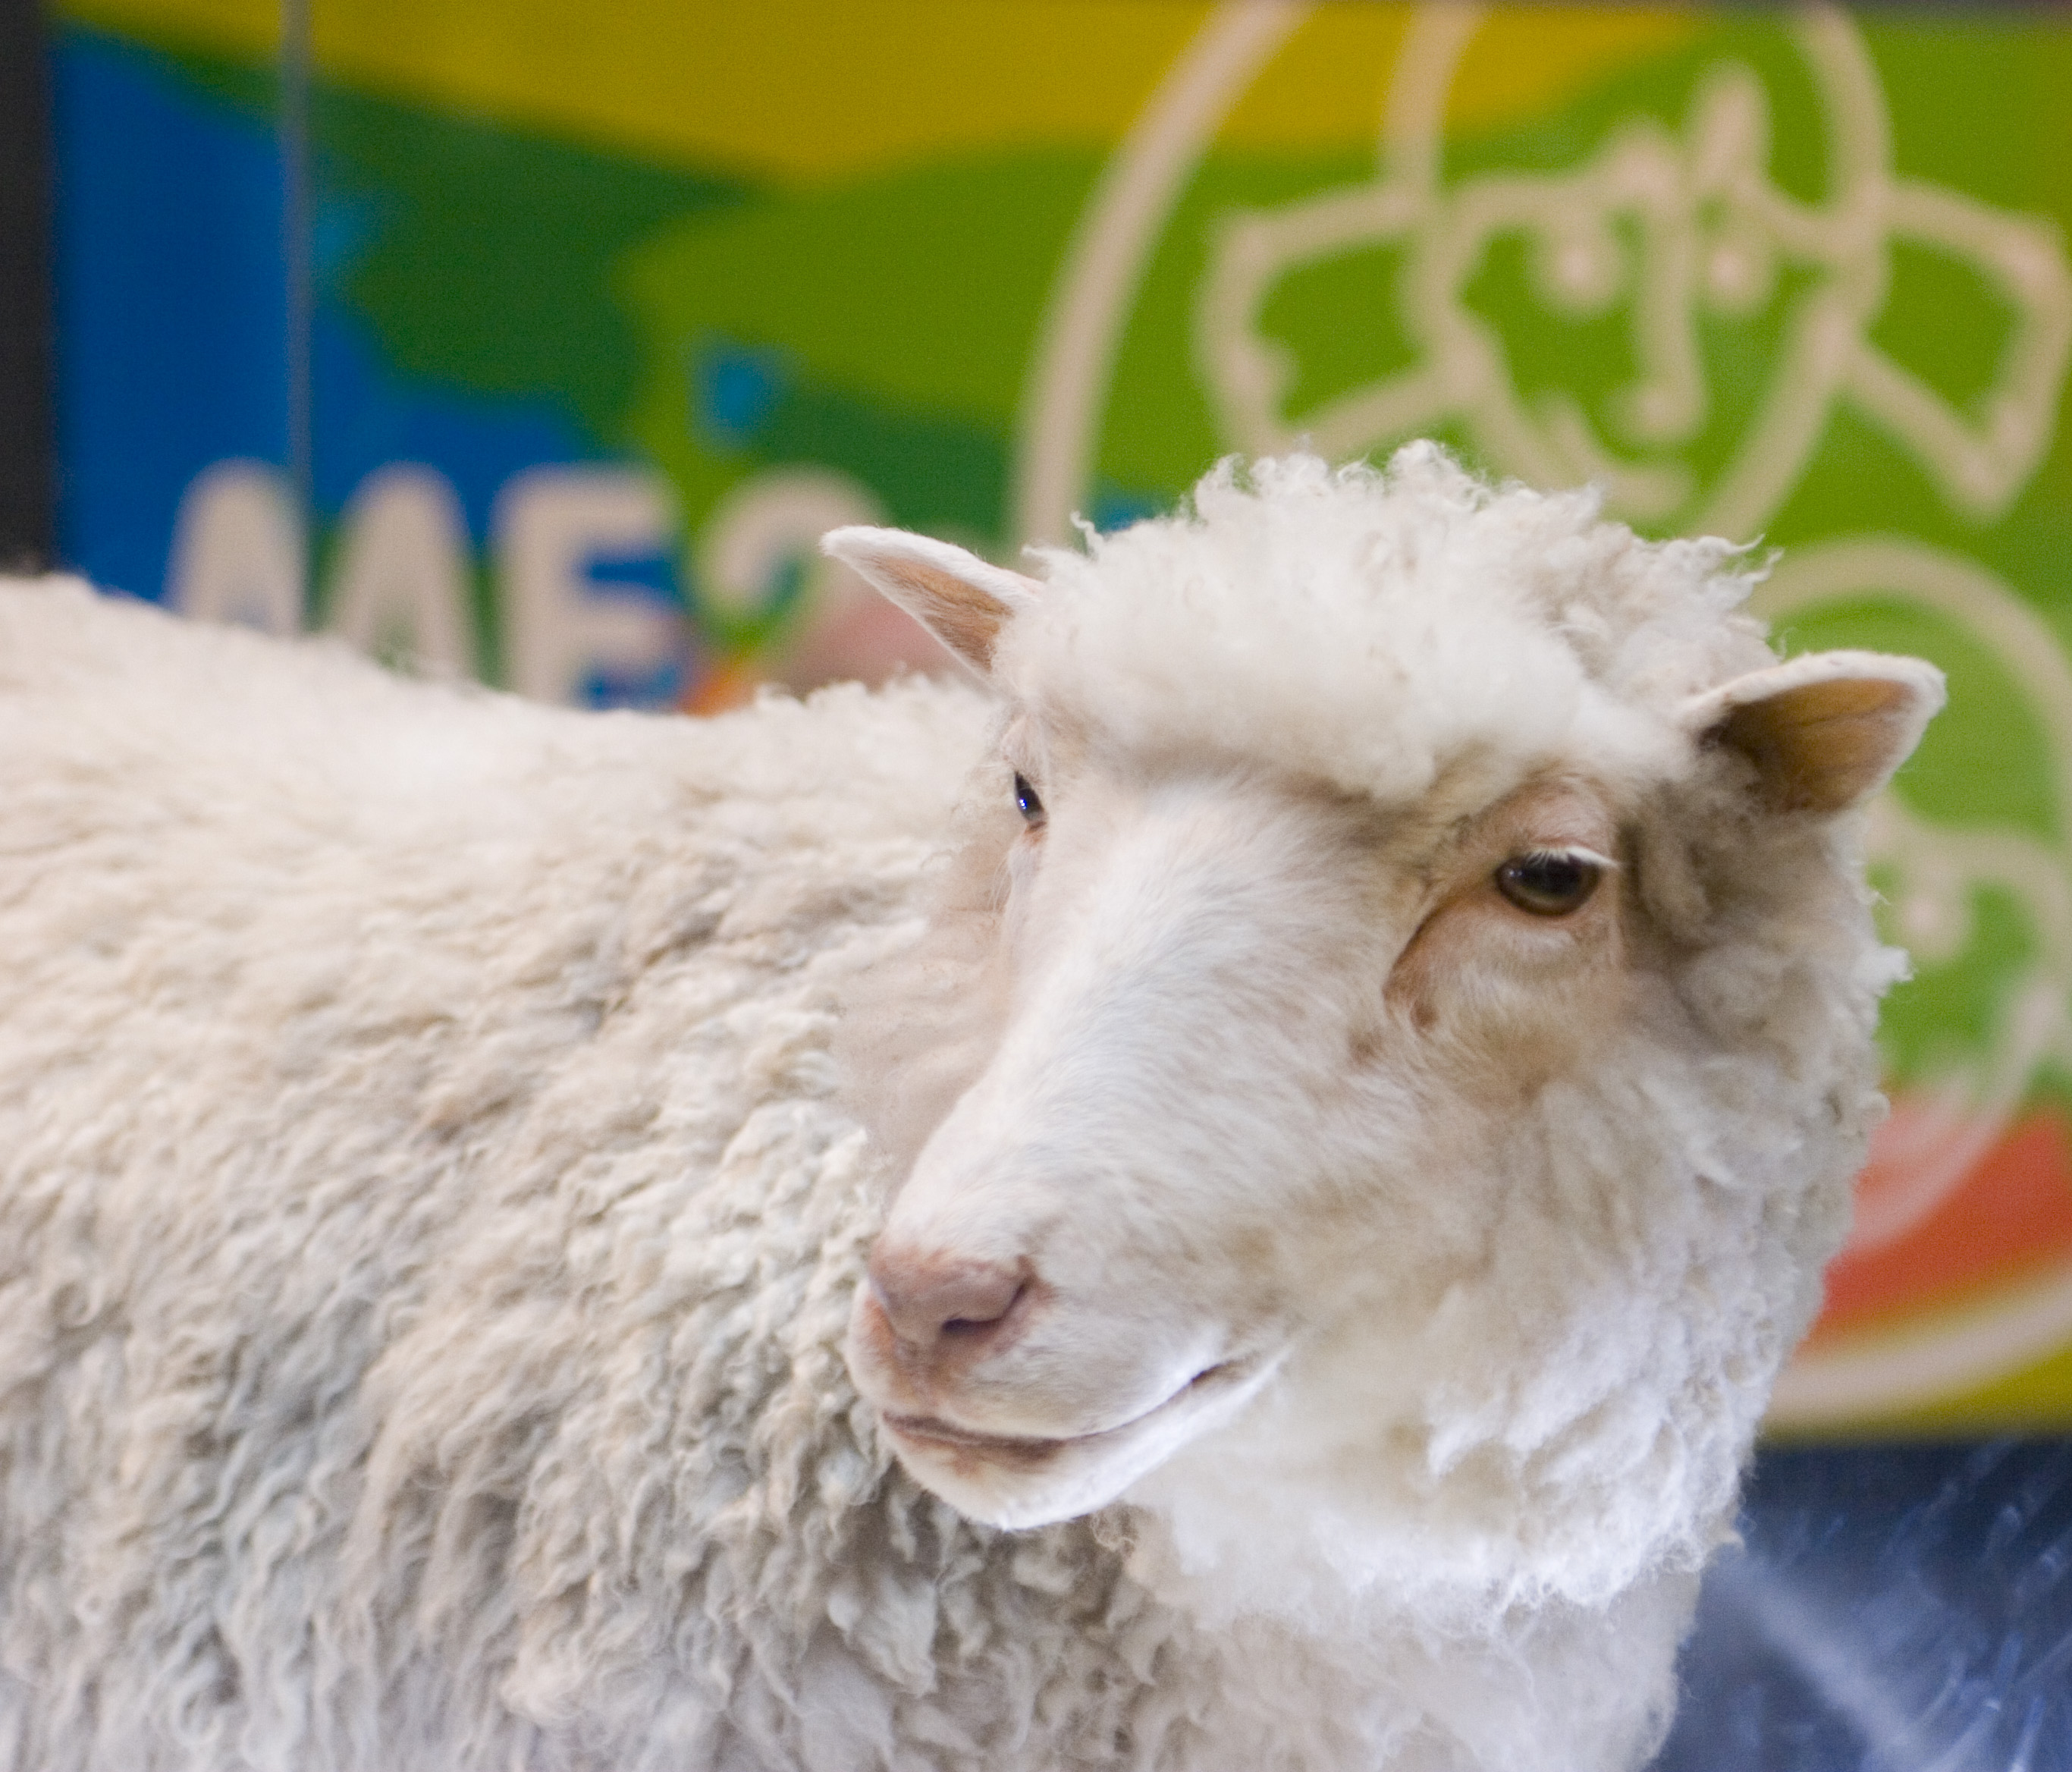
\includegraphics[width=\paperwidth,trim=0cm 0cm 0cm 5.8cm,clip]{ref/247834228_b62f7a9f65_o.jpg}}
%\setbeamercolor{title page}{fg=white}
  \begin{frame}[plain]
    \titlepage
  \end{frame}
}

%{
%\usebackgroundtemplate{%
%
\includegraphics[width=\paperwidth]{ref/micre-partners.pdf}}
%\begin{frame}{}
%\end{frame}
%}

\begin{frame}{A bit about me}
	\begin{itemize}
		\item University of New South Wales, Sydney
		\item Biostatistician and pharmacoepidemiologist
		\item Collaborating with Sabrina on \{wtdr\}
		\item Interest in causal inference methods
	\end{itemize}
\end{frame}

\begin{frame}{Outline}
	\begin{itemize}
		\item The problem
		\item Target trial specification
		\item Clone--censor--weight overview
		\item Negative controls
		\item Results
		\item Discussion
	\end{itemize}
\end{frame}

\begin{frame}{The paper}
\calculatespace%
\begin{columns}
\begin{column}{0.20\contentwidth}
\begin{tikzpicture}
  \node[drop shadow={shadow xshift=.8ex,shadow yshift=-.8ex},fill=white,draw] at (0,0) {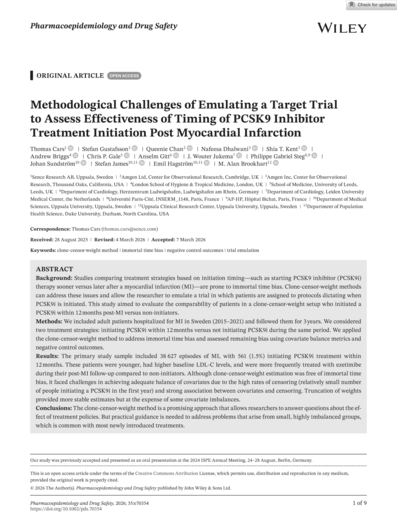
\includegraphics[width=\textwidth]{ref/cars_sm.png}};
\end{tikzpicture}
\end{column}
\begin{column}{0.70\contentwidth}
	\begin{itemize}
		\item T.~Cars, S.~Gustafsson, Q.~Chan, N.~Dhalwani, S.~.T.~Kent,
		A.~Briggs, \emph{et al.} Methodological Challenges of Emulating
		a Target Trial to Assess Effectiveness of Timing of PCSK9
		Inhibitor Treatment Initiation Post Myocardial Infarction.
		\emph{Pharmacoepidem Drug Saf}, 35(4):e70354.
		doi:10.1002/pds.70354, 2026.
\nocite{cars_2026}
	\end{itemize}
\end{column}
\end{columns}
\end{frame}

\begin{frame}{Comparative effectiveness using observational data\dots}
	\begin{itemize}
		\item Non-randomised treatment decisions \rightarrow { }bias
		\item Untreated comparator: when is time zero?
		\item Time-varying treatment \rightarrow { }time-varying confounding
		\item Intention to treat? Per protocol?
	\end{itemize}
\end{frame}

\begin{frame}{\dots is hard to do right}
%	\centering
\begin{tikzpicture}
  \node[drop shadow={shadow xshift=.8ex,shadow yshift=-.8ex},fill=white,draw] at (0,0) {
\includegraphics[height=0.3\textheight]{ref/blais-1.png}};
\end{tikzpicture}
\flushright{\begin{tikzpicture}
  \node[drop shadow={shadow xshift=.8ex,shadow yshift=-.8ex},fill=white,inner sep=0pt,draw] at (0,0) {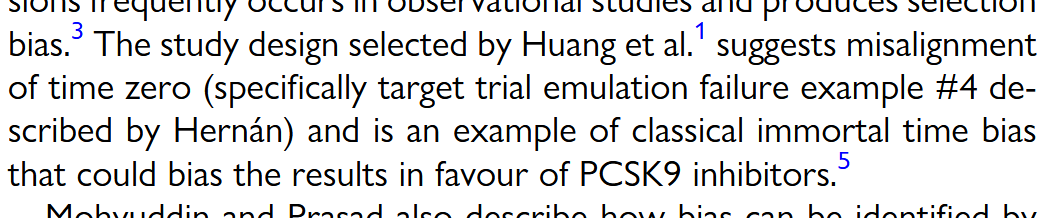
\includegraphics[height=0.3\textheight]{ref/blais-2.png}};
\end{tikzpicture}}
\flushright{\tiny{\citet{blais_2025}}}
\end{frame}
	
\begin{frame}{One solution: rigorously emulating a grace period}
	\begin{itemize}
		\item Follow \emph{everyone} from time zero
		\item Use the clone--censor--weight method
		\item Inverse probability of censoring weights maintain
			conditional exchangeability
	\end{itemize}
\end{frame}


\begin{frame}{The target trial}
	\begin{itemize}
		\item Index date: hospital discharge after MI
		\item Previously treated with a statin
		\item Treatment: Initiate PCSK9i within 12 months
		\item Control: Everyone who didn't
		\item Intention to treat (?!), three years follow up
	\end{itemize}
\end{frame}

\begin{frame}{Clone-censor-weight 1}
	\centering
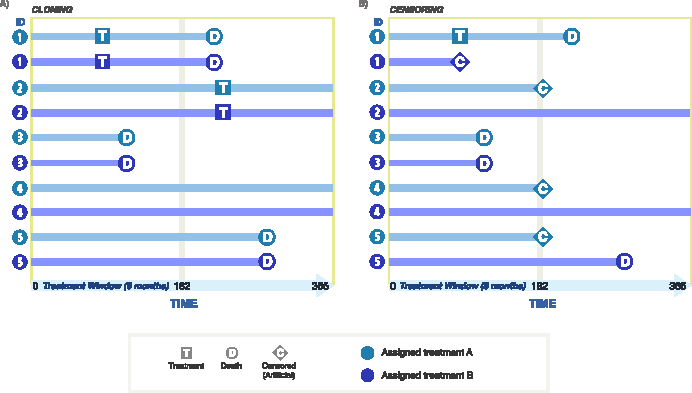
\includegraphics[height=0.8\textheight]{ref/clone-censor.pdf}
\flushright{\tiny{\citet{gaber_2024}}}
\end{frame}

\begin{frame}{Clone-censor-weight 2}
	\centering
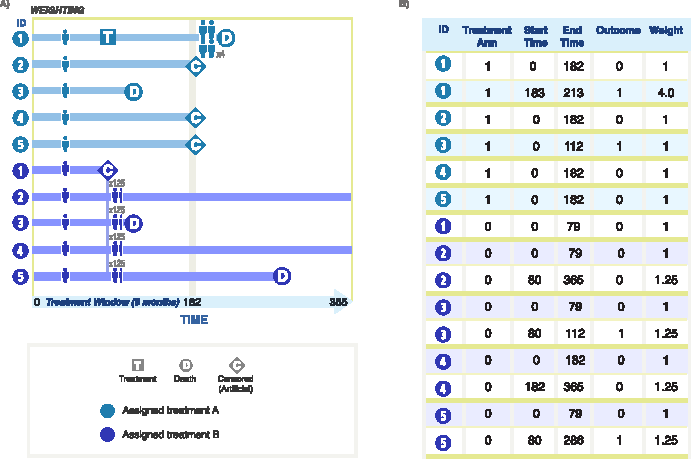
\includegraphics[height=0.8\textheight]{ref/weight.pdf}
\flushright{\tiny{\citet{gaber_2024}}}
\end{frame}

\begin{frame}[c]{WARNING!}
\centering
No ``real'' outcomes in this paper
\end{frame}

\begin{frame}{Negative control outcomes (NCO)}
\begin{columns}[T]
\begin{column}{0.5\textwidth}
	\begin{itemize}
		\item Bone fractures
		\item Hip and/or knee arthroplasty
		\item Kidney stones
	\end{itemize}
\end{column}
\begin{column}{0.5\textwidth}
	\begin{itemize}
		\item Glaucoma
		\item Non-melanoma skin cancer
		\item Other cancers
	\end{itemize}
\end{column}
\end{columns}
\end{frame}

\begin{frame}{Adjustment variables (IPCW)}
\begin{columns}[T]
\begin{column}{0.5\textwidth}
	\begin{itemize}
		\item Age and sex (b)
		\item Comorbidities (b)
		\item MI and stroke (v)
		\item Statin treatment (v)
	\end{itemize}
\end{column}
\begin{column}{0.5\textwidth}
	\begin{itemize}
		\item Ezetimibe treatment (v)
		\item LDL-C level (v)
		\item Residency (v)
		\item Calendar period (v)
	\end{itemize}
\end{column}
\end{columns}
\end{frame}

\begin{frame}{Weighting woes}
	\begin{itemize}
		\item Maximum weight 817
		\item Weights capped at 99.9th \%ile (214)
		\item Choose between bias and precision
	\end{itemize}
\end{frame}

\begin{frame}{Results: Standardised mean differences}
	\centering
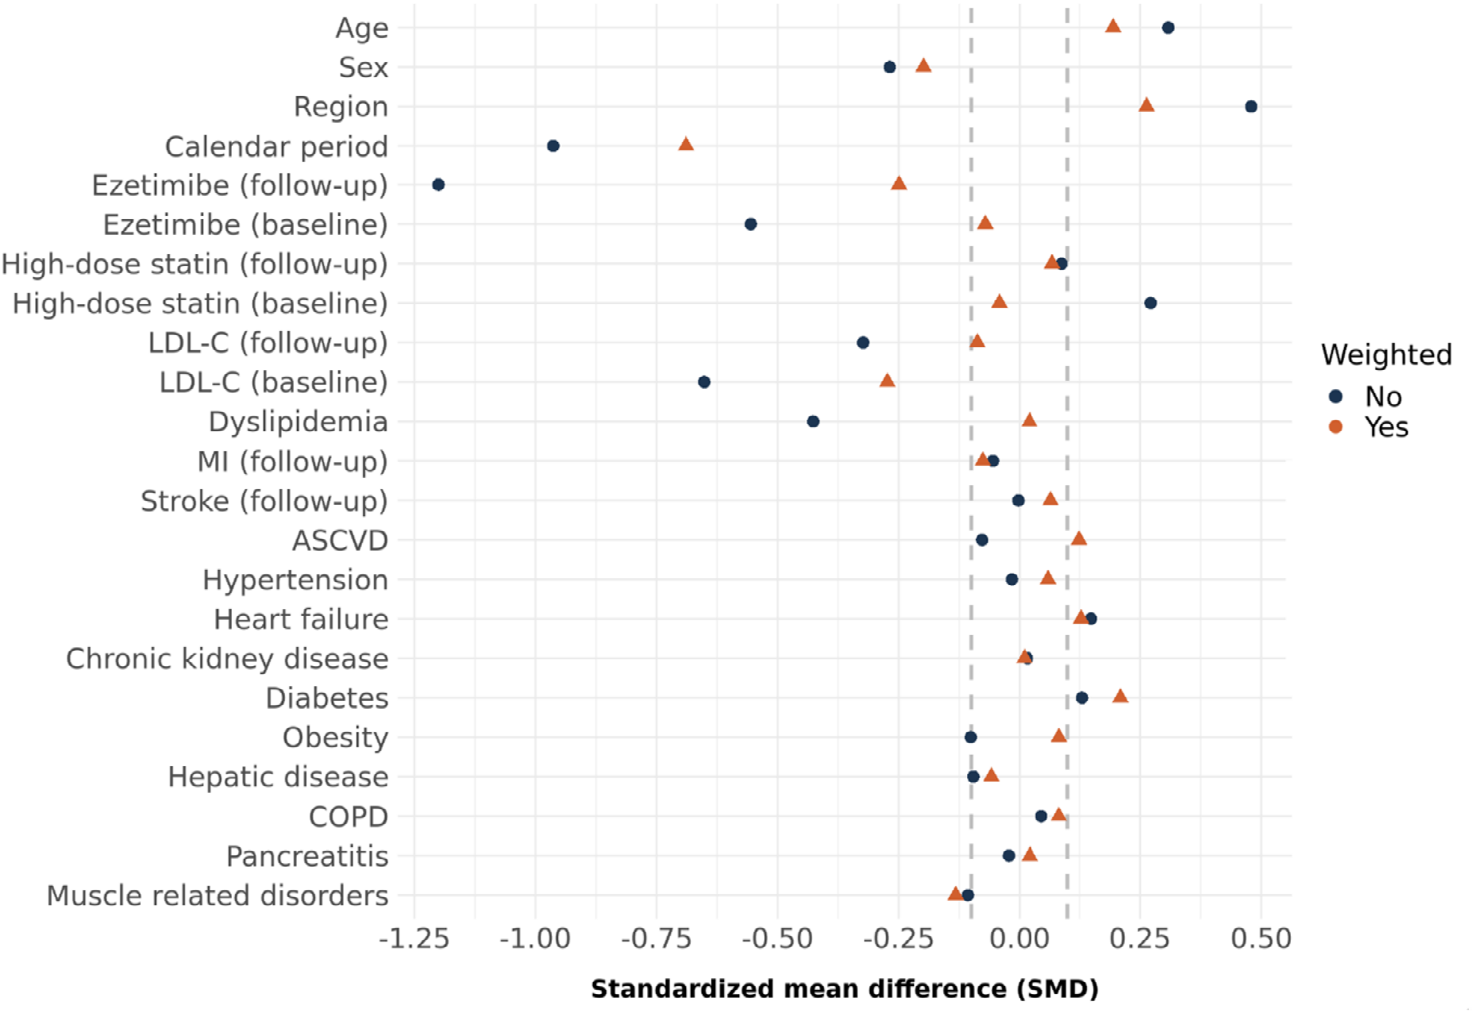
\includegraphics[height=0.85\textheight]{ref/cars-smd.png}
\end{frame}

\begin{frame}{Results: Weighted Kaplan--Meier curve}
\begin{columns}
\begin{column}{0.75\textwidth}
\centering
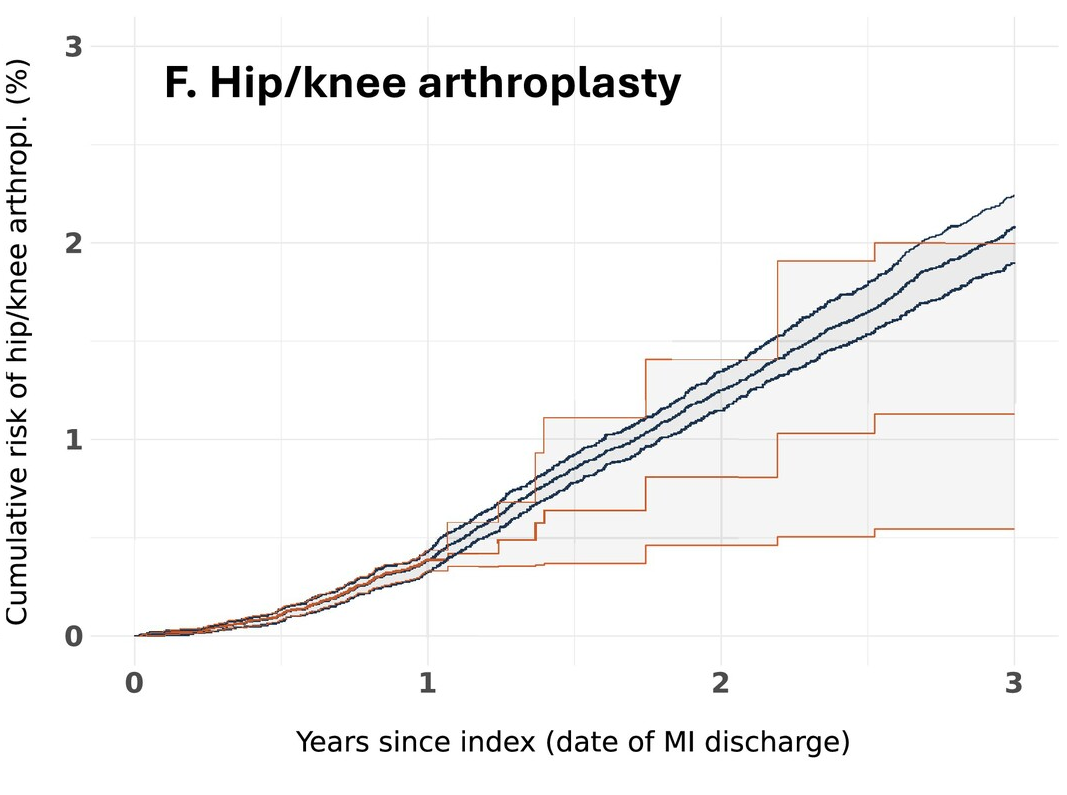
\includegraphics[height=0.85\textheight]{ref/pds70354-fig-0002f.png}
\end{column}
\begin{column}{0.25\textwidth}
HR 0.62 \\ 95\% CI 0.38--1.01
\end{column}
\end{columns}
\end{frame}

\begin{frame}{Results: Bias-variance tradeoff (fracture)}
	\centering
	\begin{tabular}{lccc}
		\toprule
		Truncation & HR & ESS (treated) & SMD >0.1 \\
		\midrule
		95th & 1.01 & 479 & 14 \\
		99th & 1.08 & 413 & 15 \\
		99.9th & 0.96 & 186 & 10 \\
		None & 0.99 & 127 & 11 \\
		\bottomrule
	\end{tabular}
\end{frame}

\begin{frame}{Summary}
	\begin{itemize}
		\item Strongly imbalanced groups
		\item Implausible effects on negative controls
		\item Similar imbalance with landmark analysis + PS
		\item Problems inherent to newly introduced treatment
	\end{itemize}
\end{frame}

\begin{frame}{Another example, this one with outcomes}
	\centering
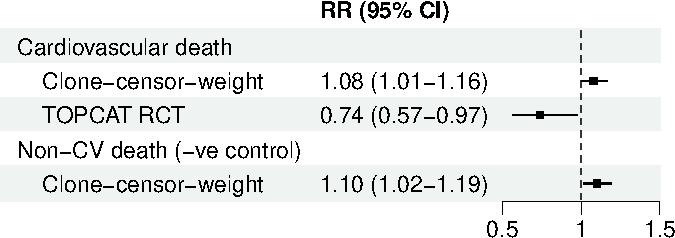
\includegraphics[height=0.5\textheight]{ref/stephan-forest-crop.pdf}
	\begin{itemize}
		\item Spironolactone vs no treatment, heart failure population
		\item Six-month grace period
	\end{itemize}
\flushright{\tiny{\citet{stephan_2026}}}
\end{frame}

\begin{frame}{Where to from here?}
	\begin{itemize}
		\item Confounding by indication is hard to fix
		\item Clone--censor--weight isn't magic
		\item Negative controls are a useful tool
		\item ACNU 4 eva?
	\end{itemize}
\end{frame}

\begin{frame}{Thank you}
    \begin{itemize}
        \item Sabrina
    \end{itemize}
\end{frame}

{
\usebackgroundtemplate{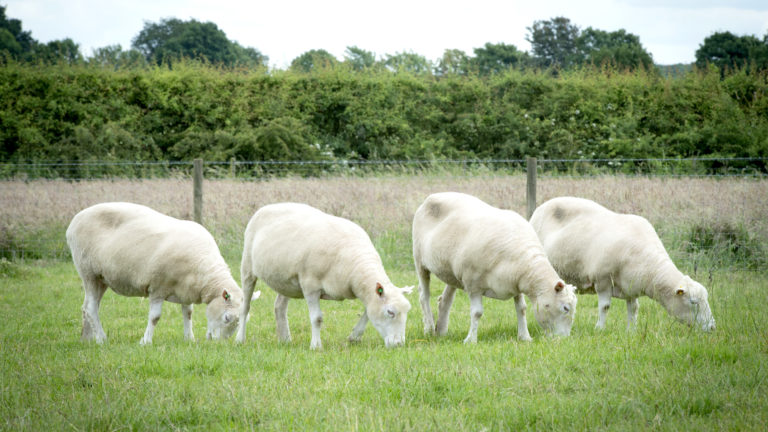
\includegraphics[width=\paperwidth,trim=0cm 0cm 0cm 0cm,clip]{ref/Nottingham-Dollies-grazing-high-res-768x432.jpg}}
  \begin{frame}{Thanks}
	\begin{minipage}[t][0.8\textheight]{\textwidth}
	    \begin{itemize}
		\item XXXX
	    \end{itemize}
	\end{minipage}
	\vfill
	\flushright{Dolly\dagger, 5 Jul 1996--14 Feb 2003}
\end{frame}
}

\begin{frame}{References}
%        \bibliographystyle{apalike}
%        \bibliographystyle{abbrv}
        \tiny\bibliography{clones.bib}
        \bibliographystyle{abbrvnat}
\end{frame}

\end{document}
